\Chapter{A dokumentum strukturális elemzése}
\label{chap:ocr}

A strukturális elemzés első lépése a beolvasott, PDF formátumú dokumentumok PNG formátumú képekké való konverziója.
A PDF formátum megválasztását az indokolta, hogy az tekinthető a leginkább elterjedt, és a legtöbb esetben átvihető formátumnak.
Az átvihetőségből egyúttal az is adódik, hogy a dokumentumban a szövegek elrendezése karakter szintjén kötött lehet, a megjelenés ugyan egységes, viszont például az egybefüggő szövegrészek kijelölése, kimásolása már problémát jelenthet.
A PNG formátum esetében szintén az elterjedtsége, szabványos kialakítása volt az egyik fő szempont, de e mellett lényeges előny, hogy tömörített és veszteségmentes módon képes tárolni a képpontok intenzitásait.

\Section{A PDF dokumentum beolvasása}

% TODO: https://pypi.org/project/pdf2image/
A dokumentumok képpé konvertálásához a \texttt{pdf2image} függvénykönyvtárt használtam [].
Ez paraméterként egyszerűbb esetben a PDF dokumentum elérési útvonalát és a kép méretét várja.
(A méret megadásánál a képarány megtartása mellett opcionális lehet a kép magassága vagy szélessége.)

% TODO: https://pypi.org/project/Pillow/
A beolvasást követően egy \textit{Pillow} [] függvénykönyvtár formátumának megfelelő képobjektum jön létre.
% TODO: NumPy hivatkozás (könyvre lehetőleg)
A \textit{Pillow} manapság már nem tekinthető korszerű eszköznek, ezért a beolvasott képeket \textit{NumPy} [] mátrixokká konvertálom.
A beolvasás és az átalakítás a \texttt{test2.pdf} esetében az alábbi módon valósítható meg.

\begin{python}
import cv2
import numpy as np
from pdf2image import convert_from_path

pil_images = convert_from_path('samples/test2pdf.pdf', size=(2500, None))
images = [
    cv2.cvtColor(np.array(pil_image), cv2.COLOR_BGR2GRAY)
    for pil_image in pil_images
]
\end{python}

A listára és a \texttt{for} ciklusra itt azért van szükség, mert a PDF több oldalt is tartalmaz (és nyilván általában tartalmazhat).

A \texttt{cvtColor} egy \textit{OpenCV} könyvtárhoz tartozó függvény, amelyik segítségével a kép szürkeárnyalatos képpé konvertálását végzem.
A strukturális elemzés alapvetően olyan kontrasztos képekre készült, amelyeknél a színek nem jelentenek lényegi információt a feldolgozás szempontjából.

\Section{Margók becslése}

Amint megvannak az oldalak, majd szürkeárnyalatos képpé alakításuk, a margók levágása következik. Az elemzés a nagyobb egységektől a kisebbek felé történik, vagyis ezt a paragrafusokra, sorokra, szavakra majd azokon belül a karakterekre vonatkozó elemzés követi majd.

Ahhoz, hogy meg tudjam állapítani, hogy hol kezdődik a szöveg, és hol található összefüggő fehér rész (margó, sorköz stb.), intenzitást kellett számolnom a kép minden sorára és oszlopára (255: fehér, 0: fekete). Ehhez átlagoltam a pixelek intenzitásának értékeit. Ezzel eredményül kaptam egy $x$ és egy $y$ tengely menti tömböt, amelyek az oszlopok és a sorok menti intenzitás átlagokat tartalmazzák.
A számítás \texttt{NumPy} segítségével egyszerűen elvégezhető.
Tegyük fel, hogy a vizsgált kép az \texttt{image} nevű változóban található.
Ekkor a sorokhoz és oszlopokhoz tartozó átlagok (profilok) a következő formában számolhatók.
\begin{python}
row_profile = np.mean(image, axis=1)
column_profile = np.mean(image, axis=0)
\end{python}
Ezt a két intenzitást \aref{fig:mf_2}. ábrával szemlélteti a program.
% amit le is ment a megadott mappába.
% TODO: A kép megjelenítési módjáról a Matplotlib kapcsán lehet írni. (axis-ok megadása)

\begin{figure}[h!]
\centering
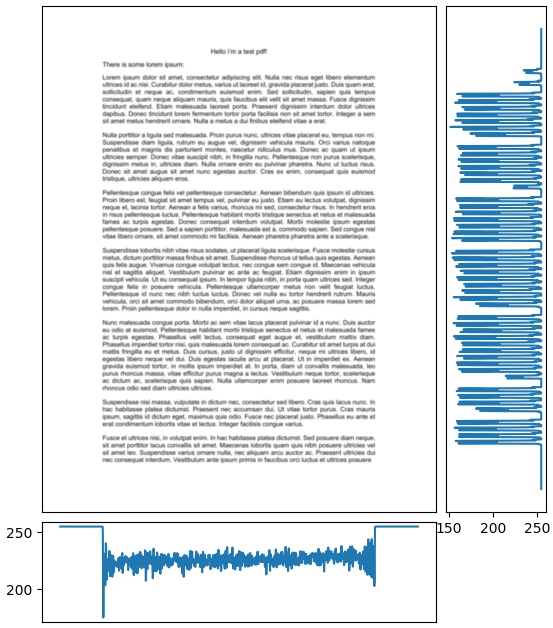
\includegraphics[scale=1]{images/mf_2.png}
\caption{A szegélyekre aggregált intenzitás értékek}
\label{fig:mf_2}
\end{figure}

Ezt a két tengely menti intenzitás tömböt felhasználva már meg lehet állapítani, melyik pixelnél ér véget a margó és hol kezdődik a szöveg. Egy egyszerű ciklussal megvizsgálom a tömb elejétől indulva hogy meddig egyenlőek az intenzitások a 255 értékkel, majd lementem azt az indexet ahol megáll a programom. Ezt megismétlem a tömbön visszafelé haladva is, így lesz meg az alsó-felső, jobb-bal margó végpontja. Ezeket felhasználva a programom már tudja kezelni a paragrafusokat tartalmazó képterületet.

A változás helyének detektálását \texttt{find\_first\_change} és a \texttt{find\_last\_change} függvények végzik.
Ezek a következőképpen kerültek megvalósításra.
\begin{python}
def find_first_change(values):
    """
    Find the index of the first changed value in the values.
    :param values: an iterable array of comparable objects
    :return: the i index where values[i - 1] != values[i]
    """
    i = 1
    while i < len(values):
        if values[i - 1] != values[i]:
            return i
        i += 1
    raise ValueError('All values are the same!')
\end{python}

\begin{python}
def find_last_change(values):
    """
    Find the index of the last changed value in the values.
    :param values: an iterable array of comparable objects
    :return: the i index where values[i] != values[i + 1]
    """
    i = len(values) - 2
    while i >= 0:
        if values[i] != values[i + 1]:
            return i
        i -= 1
    raise ValueError('All values are the same!')
\end{python}

A képek kiemelt fontosságú részét \textit{Region of Interest} (röviden ROI) néven szokta emlegetni a szakirodalom. A programomban ezen területek adatainak kezeléséhez egy \texttt{Region} osztályt definiáltam, amely \textit{(sor, oszlop, sorok száma, oszlopok száma)} négyessel jellemzi a téglalap alakú területet.

Ezek segítségével a margók a következő formában számolhatók.
\begin{python}
def calc_margins(image):
    """
    Calculate the margins of the image.
    :param image: the NumPy array of page intensity image
    :return: a Region instance
    """
    row_profile = np.mean(image, axis=1)
    column_profile = np.mean(image, axis=0)
    row = find_first_change(row_profile)
    column = find_first_change(column_profile)
    n_rows = find_last_change(row_profile) - row
    n_columns = find_last_change(column_profile) - column
    margins = Region(row, column, n_rows, n_columns)
    return margins
\end{python}
Az ilyen formában becsült margókat a \texttt{matplotlib} függvénykönyvtár segítségével visz\-sza is lehet rajzolni a képre.

% TODO: Esetleg beletenni a margós megjelenítést végző kódrészt és az eredményét.

\Section{Paragrafusokra bontás}

A paragrafusokra bontásnál feltételezés az, hogy a dokumentumnak van egy adott háttérszíne. Ez ugyanaz az érték, amely a kép széleinél megjelenik (vagyis a margók kereséséhez is felhasználásra került). Nyilvánvalóan ez a dokumentumok jelentős részében fehér, vagyis szürkeárnyalatos skálán a 255 intenzitásértéknek felel meg.

A sorokra bontásnál azt a tulajdonságot használhatjuk fel, hogy a soronként vett átlagintenzitások kisebbek (az áltagos szín sötétebb), mint a sorok között (\ref{fig:line}. ábra).

\begin{figure}[h!]
\centering
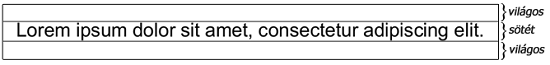
\includegraphics[scale=1]{images/line.png}
\caption{A jellemző átlagintenzitások a soronként vett profilban}
\label{fig:line}
\end{figure}

A paramgrafusok elkülönítésénél az a cél, hogy a nem háttérszínhez tartozó szakaszok ki legyenek gyűjtve.
A Python kód ez esetben is könnyen áttekinthető, annak a működését a következő kódrészben láthatjuk.
\begin{python}
def find_segments(values, background_color):
    """
    Find the segments with non-background colors in the iterable.
    :param values: intensity values
    :param background_color: the background color which should be skipped
    :return: list of segments as [start, end) tuples of indices
    """
    segments = []
    start = None
    end = None
    for i, value in enumerate(values):
        if value != background_color:
            if start is None:
                start = i
        elif start is not None:
            end = i
            segments.append((start, end))
            start = None
    return segments
\end{python}

% TODO: Esetleg bele lehet tenni a megjelenítéshez használt kódrészt és a kijelölt paragrafusokat.

Jelenleg feltételezzük, hogy olyan dokumentumbról van szó, amelyben a sorok és a paragrafusok közötti távolságok különböznek.
Ennek vizsgálatához gyűjtsük ki a paragrafusok között lévő távolságokat, majd vizsgáljuk meg azok eloszlását! A gyakorisághisztogram \aref{fig:segment_hist}. ábrán látható.

\begin{figure}[h!]
\centering
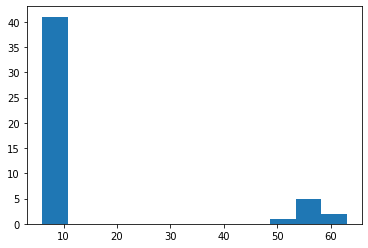
\includegraphics[scale=1]{images/segment_hist.png}
\caption{A sorok és paragrafusok közötti távolságok eloszlása.}
\label{fig:segment_hist}
\end{figure}

Jól látható, hogy tartomány közepén nincsenek értékek, így például egy 30 képpontnyi küszöbérték megfelelő az elkülönítéshez.

A szegmensek (mint nem háttér színű összetartozó részek) elkülönítésénél balról zárt, jobbról nyitott intervallumok szerepeltek.
Ezeket egy külön függvény segítségével érdemes egymáshoz kapcsolni, abban az esetben, hogy ha a távolságuk nem haladja meg az adott minimális távolságot.
Az alábbi kódrészlet ezt a feladatot látja el.
\begin{python}
def join_segments(segments, min_spacing):
    """
    Join the segments which are closer to each others
    than the minimal spacing.
    :param segments: list of segments as [start, end) intervals
    :param min_spacing: the minimal spacing between the joined segments
    :return: list of segments in the same format as the input
    """
    joined_segments = [segments[0]]
    for segment in segments[1:]:
        if (segment[0] - joined_segments[-1][1]) < min_spacing:
            joined_segments[-1] = (joined_segments[-1][0], segment[1])
        else:
            joined_segments.append(segment)
    return joined_segments
\end{python}
Az eredmény megjelenítéséhez a \texttt{matplotlib} például az alábbi formában biztosít eszközöket.
\begin{python}
margins = calc_margins(image)
row_profile = np.mean(image, axis=1)
background_color = 255
segments = find_segments(row_profile, background_color)
fig, ax = plt.subplots(figsize=(10, 20))
plt.imshow(image, cmap='gray')
for segment in joined_segments:
    n_rows = segment[1] - segment[0]
    rectangle = plt.Rectangle(
        (margins.column, segment[0]), margins.n_columns, n_rows,
        facecolor='red', alpha=0.1)
    ax.add_patch(rectangle)
plt.show()
\end{python}
Ez az eredeti képen kijelöli a kigyűjtött paragrafusokat (pontosabban azokat a részeket, amelyek a jelenlegi változat szerint a távolság alapján paragrafusként detektálhatók).

\begin{figure}[h!]
\centering
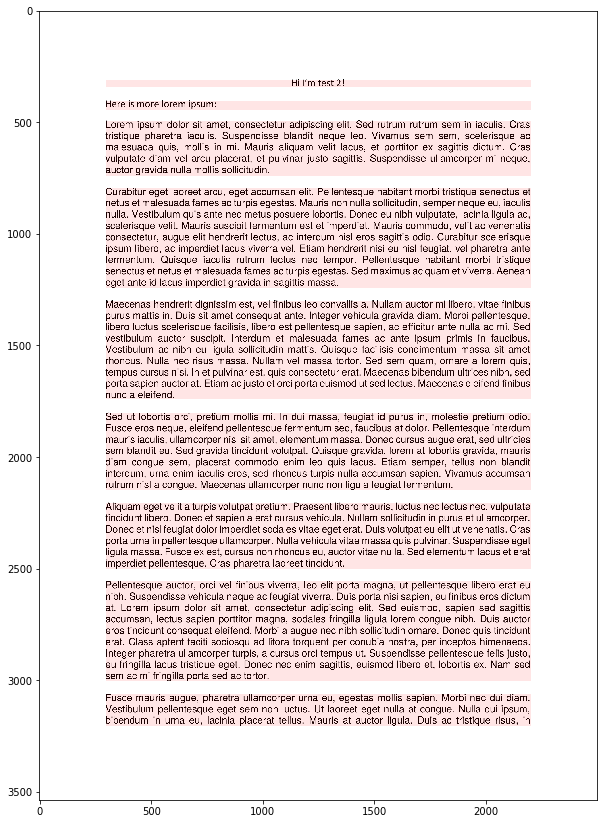
\includegraphics[scale=0.6]{images/highlighted_paragraphs.png}
\caption{A program által megtalált és kijelölt paragrafusok.}
\label{fig:highlighted_paragraphs}
\end{figure}

Amennyiben a szövegen kívül más nem szerepel az adott oldalon, a sorokra bontáshoz nem szükséges, hogy az adott oldalt felbontsuk paragrafusokra, az eredeti képből könnyedén megkaphatjuk a sorokat. Viszont, ha nem csak szöveges részeket tartalmazó dokumentummal van dolgunk, abban az esetben a sorokra bontás előtt szükséges megvizsgálni, hogy az oldal mely részei tartalmaznak szöveget, és mely részei tartalmaznak egyéb elemeket (például képeket vagy táblázatokat). Ezt a problémát majd a dolgozat későbbi részében fejtem ki bővebben.

\Section{Szavakra bontás}

A szavakra bontásnál szükségem van az eddig levágott sorokra, így egy \textit{for} cikluson belül egyesével beolvasom őket, majd első lépésként kigyűjtöm a szavak koordinátáit. Itt már nem az $y$, hanem az $x$ tengely menti intenzitást használom fel, és az előző algoritmusokhoz hasonlóan a világos, 240 feletti intenzitást keresem, és amint találok belőle egymás mellett legalább 5 darabot, akkor mentem le a koordinátát. Mivel a világos részek érzékelésével keresem a szavakat, így a legelső szó elején is kell hogy legyen valamennyi világos terület hogy ne hagyja ki az algoritmus a vizsgálat során. Emiatt nem vágom le a soroknak a bal részéről a margót, mivel így biztosan megtalálja az összes szót. A másik megoldás az lehetne, hogy automatikusan lementem a 0 indexet, mint kezdőindex, ezzel is biztosítva hogy a kezdeti szó koordinátái is meglegyenek, de úgy véltem hogy a margó elhagyása egy logikusabb lépés.

\Section{Karakter szintű elemzés}

A szavak betűkre bontása már egy érdekesebb témakör. Ennél az algoritmusnál már nem a világos, hanem épp hogy a sötét részeket kerestem, és ha már 1 pixelnek megfelelő sötét részt is találtam már mentettem az adott indexet. Ez a legtöbb esetben szépen működött, és megkaptam egyesével a betűket. Viszont a ligatúrák esetében a betűk egymásba lógnak, ezért az algoritmusom nem vágta szét őket, hanem egybe mentette le. Ilyen esetek voltak például az \emph{r} és az \emph{f} vagy \emph{t} találkozása, vagy például a dupla \emph{t} vagy \emph{f} betűk.

\Section{Bonyolultabb dokumentumok}

Az eddigiekben azt feltételeztük hogy a dokumentum amelyet vizsgálunk, az szövegen kívül mást nem tartalmaz, és az adott szöveg is folytonos, egyetlen hasáb. Amennyiben egy bonyolultabb szerkezetű PDF dokumentumot kell feldolgoznunk (például amely sematikus vázlata \aref{fig:page}. ábrán látható), abban az esetben az eddigi algoritmusok a paragrafusokra bontásig működnek, ám az esetlegesen előforduló képeket és a táblázatokat nem kezeljük külön, abban az esetben a sorokra bontásnál a folyamat megszakad. Annak érdekében, hogy ezt elkerüljük, a paragrafusokra bontásnál egyéb vizsgálatokra van szükség.

\begin{figure}[h!]
\centering
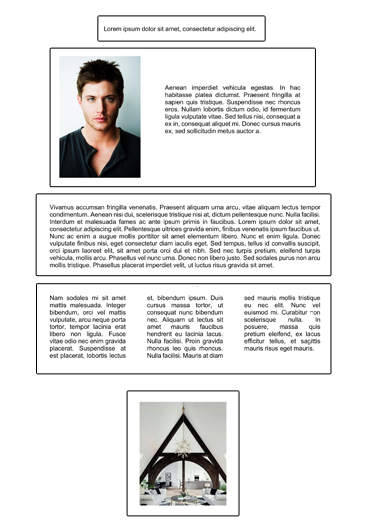
\includegraphics[scale=0.8]{images/page.png}
\caption{Nem csak egyszerű szöveget tartalmazó dokumentum sematikus vázlata}
\label{fig:page}
\end{figure}

A paragrafusra bontás során a vizsgálat az $y$ tengely mentén történik. A képek amelyeket ez úton megkapunk, vízszintesen bontják részekre a dokumentumot, tehát ha több hasábunk, vagy netalántán egy képünk van mellette valamennyi szöveggel, azok mind egy egységet alkotnak. A feladatunk hogy ezeket az egységeket szétbontsuk, és megismerjük hogy az adott részegységek szöveget tartalmaznak vagy valami mást. (A felbontás első nagyobb lépésének eredményét \aref{fig:page2}. ábrán láthatjuk.)

\begin{figure}[h!]
\centering
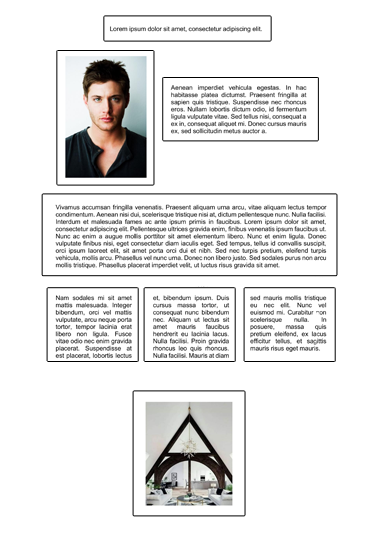
\includegraphics[scale=0.8]{images/page2.png}
\caption{Az egységekre bontás első szakaszának eredménye}
\label{fig:page2}
\end{figure}

A további szétbontás hasonlóan működik, mint az eddigi algoritmusok. Betöltjük magát a képet, végrehajtunk rajta egy intenzitás vizsgálatot méghozzá az $x$ tengely mentén, majd ezt megvizsgálva kimentjük a fehér részek koordinátáit. (Az eredmény szemléltetése \aref{fig:page3}. ábrán látható.)

\begin{figure}[h!]
\centering
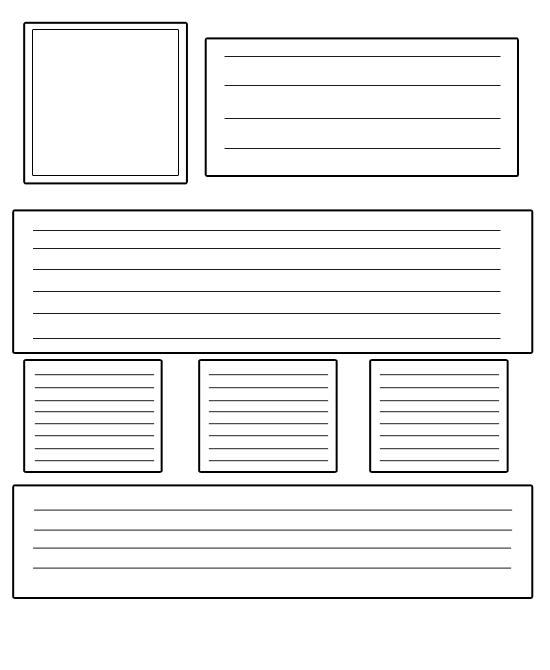
\includegraphics[scale=0.8]{images/page3.png}
\caption{Az egységekre bontás második szakaszának eredménye}
\label{fig:page3}
\end{figure}

Abban az esetben, ha az algoritmus nem talál koordinátát, akkor visszatér egy hamis értékkel, és a teljes képpel dolgozik tovább.

Amennyiben talál, akkor következik a részegységekre bontás. Mivel a paragrafusoknál a bal és jobb szélső margó már nem kerül figyelembevételre a képen, így nincsen kezdeti fehér rész amelyből az algoritmus kiindulhatna. Ezért a koordinátákat tartalmazó lista kezdő, és végpontja a margókon belüli rész kell legyen. Ezt a két értéket a kivágáshoz használt (\texttt{crop}) metódus előtt hozzáadom a listához. 

Amennyiben a kép vagy szöveg tartalmaz behúzást, abban az esetben az algoritmus megtalálja a jobb/bal oldali fehér részt, így a kezdeti és végpont hozzáadása már nem szükséges mivel a lista már tartalmazza azokat. Egy egyszerű elágazással meg tudom állapítani, hogy szükséges-e a hozzáadás vagy sem. Ezt a megoldást a későbbiekben bevezettem a szavakra bontásnál is, hiszen így nem kell üres területeket kihagynom a sorokra bontás során.

Eredményül a program visszaadja a dokumentumot egységekre bontva. Ezek után már csak azt kell megvizsgálni, hogy az adott egység kép vagy szöveg, és ennek megfelelően menteni.

\Section{Képek és szövegek megkülönböztetése}

A vizsgálathoz azt a tényt használtam fel, hogy ha a szöveg akár csak egy sorból is áll, alatta és felette mindenképp található világos intenzitás (nem biztos hogy teljesen fehér, hiszen a szöveg vonala alá érő betűknek, mint például a \emph{p}, a szára beletartozik az adott intenzitásba így az már nem csak 255-ös intenzitásértékeket tartalmaz). Az algoritmus világos intenzitást keres elsőnek. Amint talál legalább 2 egységnyi világos területet (240 feletti intenzitás), abban az esetben az adott ponttól elindul, és megnézi hogy talál-e egybefüggő sötét területet (240 alatti intenzitás). Amennyiben igen, megvizsgálja, hogy a sötét intenzitású terület után talál egy újabb fehér részt. Amennyiben erre is az a válasz hogy igen, az algoritmus arra a következtetésre jut, hogy az adott egység szöveget tartalmaz, így azt a paragrafusokhoz menti, egyébként pedig a képekhez. Természetesen az algoritmus elég kezdetleges, így könnyen át lehet verni egy világos hátterű, középen sötét árnyalatú objektumot tartalmazó képpel (lásd \ref{fig:tree}. ábra).

\begin{figure}[H]
\centering
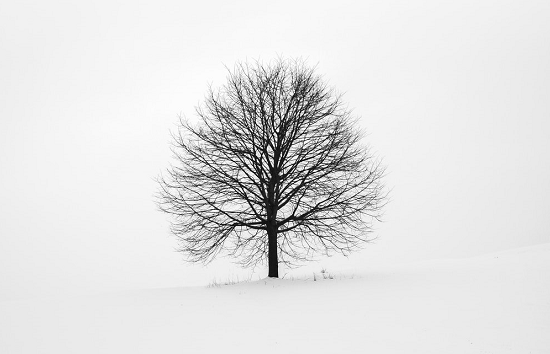
\includegraphics[scale=1]{images/tree.png}
\caption{Az algoritmus ezt a képet szövegként érzékeli}
\label{fig:tree}
\end{figure}

Az eddigi feldolgozás során a dokumentumot alulról-felfelé bontottuk részekre, viszont ahhoz, hogy végeredményként értelmes szöveget kapjunk, elengedhetetlen hogy a képek az oldalon való előfordulás szerinti sorrendben legyenek lementve.

Mivel az intenzitás vizsgálat a lap aljáról indul, így a lista pont fordított sorrendben tartalmazza a koordinátákat. Eddig a \texttt{crop} metódusban a \textit{for} ciklusom a lista elejéről, most viszont a lista végéről indul el, így a lap tetején lévő paragrafus lesz lementve elsőnek, nem pedig a lap alján levő. A paragrafusokon kívül a sorok crop metódusát kellett még módosítanom, a szavakét, és a karakterekét nem, mivel azokat az $x$ tengely mentén vágom, így azok eleve megfelelő sorrenbe kerültek mentésre.

Ezzel a dokumentumom fel van bontva a legapróbb egységre (karakter) és megfelelő sorrendben követik egymást az egységek, így következhet a karakterek felismerése \textit{Optical Character Recognition} (röviden OCR) segítségével.

\Section{Karakterek felismerése}

A Python egyik leginkább elterjedt OCR eszközét, a \textit{Python-tesseract}-ot választottam.
% TODO: Tesseract hivatkozás!
Első lépésben a karakter levágásnál átadtam a \texttt{pytesseract} \texttt{image\_to\_string} nevű metódusának a képet, majd a válaszként kapott sztringet hozzáfűztem egy már meglévő sztringemhez. Amint végig ért a metódus minden soron, egy külső állományba lementettem a megkapott szöveget. Ezen első próbálkozásnál sajnos azt tapasztaltam, hogy az OCR egyetlen karaktert sem ismert fel.

Ebből arra következtettem, hogy a felbontása az adott képnek túl alacsony lehet, így megpróbálkoztam egy nagyobb felbontású képpel, de sajnos úgy sem jártam sikerrel.

Következő lépésként egy szintet visszább léptem, és most nem a karaktereket, hanem a szavakat adtam át a metódusnak. Itt már sokkal kielégítőbb eredményt kaptam. A szavakat nagyjából 80\%-os pontossággal beazonosította, viszont itt is akadtak problémák bőven. Az egy és két betűs szavakat/kötőszavakat (például \emph{az}, \emph{és}, \emph{a}, \emph{s}) és a számokat nem ismerte fel a metódus (vagy csak nagyon ritkán), és üres szövegeket kaptam helyettük. Ezen kívül elég sok ékezet lemaradt, és gyakran keverte a betűket, például az \emph{I} és az \emph{l} esetében.

Ezen tapasztalataim után nekiláttam az OCR paramétereinek a vizsgálatához, és néhány beállítással sikerült elérnem hogy az OCR működjön karakter szinten is. Ehhez a paraméterek változtatása mellett biztosítottam, hogy az általam kivágott betűk körül mindig legyen egy fehér színű, 10 képpont méretű keret, ezzel segítve a programot a sikeresebb felismerésben. A betűtípustól függően akadnak itt is kisebb-nagyobb hibák. A word alapértelmezett \textit{Calibri} betűtípusában szereplő \emph{l} betű az tulajdonképpen egy vonal, így azt a program a | (AltGr + W) karakterként ismeri fel. Emellett gyakran összetéveszti a \emph{c} betűt az \emph{e} betűvel, a vesszőt pedig a ponttal.

Ezek természetesen az eddigi hibákhoz képest sokkal biztatóbb eredmények, és így a kapott szöveg már olvasható.

A különböző szöveg szerkezeti egységeken való OCR használat kapcsán elvégeztem néhány tesztet. Megvizsgáltam, hogy az adott szinteken (oldal, bekezdés, sor, szó, karakter) milyen időkülönbséggel fut le a karakterfelismerő. Minden esetben \aref{fig:mf_2}. ábra PDF dokumentumát használtam bemenetként. Ez egy egy oldalas dokumentum amely 672 szót és 4520 karaktert tartalmaz. Az eredmény \aref{fig:test_ocr}. ábrán lévő grafikonon látható.

\begin{figure}[h!]
\centering
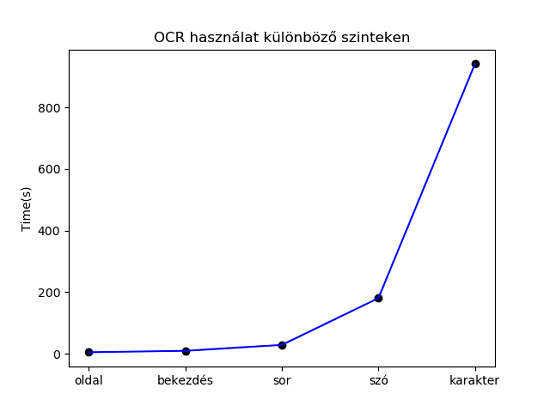
\includegraphics[scale=1]{images/test_ocr.png}
\caption{Az OCR futásának ideje másodpercben különböző szöveg szerkezeti egységeken}
\label{fig:test_ocr}
\end{figure}

Amikor az OCR egy nagyobb egységet kapott feldolgozásra, akár egybe egy oldalnyi szöveget, egy bekezdést vagy csak egy sort, csekély, mindössze 5-20 másodperces különbséggel már vissza is adta az eredményt. Viszont amikor már kisebb egységekkel volt dolga, sokkal több időbe telt neki mire megtalálta a legmegfelelőbb karakter. A szavaknál már olyan átlag 180 másodpercet, míg a karaktereknél ez olyan átlag 930 másodpercet vett igénybe.

Ez a különbség főként abból adódhat, hogy bizonyos karaktereknél szüksége van az OCR-nek viszonyítási alapra, önmagában nem tudja biztosan megmondani hogy milyen karaktert kapott. Tegyük fel hogy beadunk neki egy kis \emph{v} betűt. Ha nincs mellette viszonyítási alap, tegyük fel egy \emph{a} betű, akkor a \emph{v} az lehet kicsi és nagy betű is. Viszont ha már egybe látja az OCR a kettő betűt, \emph{av} akkor már megtudja állapítani hogy a karakter az kicsi. Tapasztalatom szerint ez a szavak szintjén sem kielégítő, viszont a sorok szintjén már elég nagy pontossággal megtudja különböztetni a kis- és nagybetűket.

A tesztet elvégeztem különböző betűtípusok esetén (\textit{Calibri}, \textit{Arial}, \textit{Times New Roman}). Arra a kérdésre kerestem a választ, hogy megnehezítik-e a feldolgozást bizonyos betűtípusok vagy sem. Mint az \aref{fig:test_font}. ábrán látható, nem nagy az eltérés a különböző betűtípusok feldolgozása között. A három példa közül az \textit{Arial} volt aminek a kiértékelése több időt vett igénybe minden szöveg szerkezeti egységen, de ez is nagyon csekély eltérés, így az ábrán nem is szembetűnő.

\begin{figure}[h!]
\centering
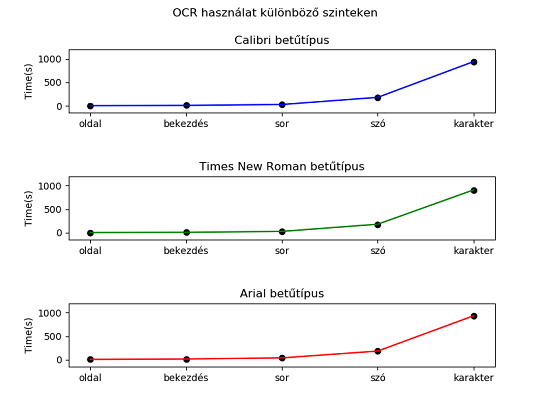
\includegraphics[scale=1]{images/test_ocr_font_types.png}
\caption{Az OCR futásának ideje különböző betűtípusok esetén}
\label{fig:test_font}
\end{figure}

Azon kívül, hogy a feldolgozása a nagyobb szöveg egységeknek gyorsabb, a tesztek során az is kiderült, hogy pontosabb is. Ez első sorban a már fentebb említett karakterek egymáshoz való viszonyításának köszönhető, hiszen itt bőven akad betű amihez viszonyíthatjuk a többit. Azért a karakterek szintjén történő OCR használatát sem kell kizárni a lehetőségek közül, mivel annál is minden esetben 75\% feletti volt az eredmény pontossága. Itt a legtöbb hibát a fentebb említetten kívül az okozza, hogy különböző betűtípusokban találhatók egymásra nagyon hasonlító betűk.

\Section{Küszöbértékek meghatározása}

Eddig tapasztalati küszöbértéket használtam a sorok és a paragrafusok elkülönítésére. Mivel minden dokumentumnak más térközei, betűméretei lehetnek így ez nem megfelelő minden PDF-re. Ezért mielőtt megkezdeném a dokumentum feldolgozását, meghatározom az adott értékeket azokat használom fel a számítások során.

Az $y$ tengely menti intenzitást vizsgálom, méghozzá azon belül is az összefüggő világos (háttér) intenzitásokat keresem. Amint más intenzitást találok, abban az esetben az eddigi összefüggő rész nagyságát lementem, majd a számolást újra kezdve haladok tovább. Eredményül egy listát kapok ami tartalmazza a térközök nagyságát.

\Aref{fig:mf_2}. ábrán szereplő dokumentum ilyen módon kiszámított térközeinek eloszlása \aref{fig:spacing} ábrán látható.

\begin{figure}[h!]
\centering
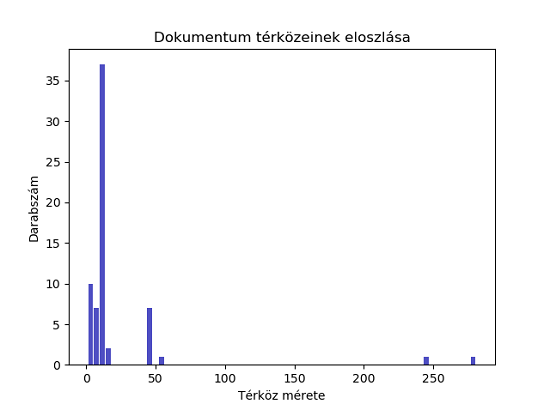
\includegraphics[scale=1]{images/spacing.png}
\caption{\Aref{fig:mf_2}. ábrán szereplő dokumentum térközeinek eloszlása}
\label{fig:spacing}
\end{figure}

Az ábrából jól kivehető hogy 3 fő csomópontja van a térközöknek. A bal szélső a sorköz, a középső a bekezdés majd az utolsó a margó. Ezen csomópontok kezdeti értéke között mindig legalább 10 lesz a  különbség, ezt használom fel a küszöbértékek meghatározásához. Miután megkaptam az adott nagyságokat, a \texttt{collections} könyvtár \texttt{Counter} metódusával rendezem őket, így megkapom, hogy milyen nagyságú intenzitásból mennyi van összesen a dokumentumban. Ezeket növekvő sorrendbe rendezem. Elindítok egy ciklust, és a 3-nál nagyobb elemeket vizsgálom, mivel a 3 és a kisebb nagyságú térköz nagy valószínűséggel csak zaj. Az első elemet lementem küszöbértéknek, majd tőle elindulva egy új ciklussal addig vizsgálom az térköz nagyságokat amíg nem lesz nagyobb a kettő különbsége mint 10. Amint ez igaz, az eddigi küszöbértéket lementem egy listába, és az utoljára vizsgált érték lesz az új küszöböm.

Végeredményül kapok egy listát, ami \aref{fig:spacing}. ábrán látható csomópontok kezdeti értékét tartalmazza. Ennek a listának a 0. eleme lesz a sorköz, az 1. eleme a térköz és a 3-4. eleme pedig az alsó-felső margó.

\Section{Képfelismerés neurális háló segítségével}

A programom fő része maga a paragrafusokra bontás, és az ilyenkor történő képfelismerés. Ekkor dönti el a program hogy érdemes-e az adott résszel foglalkozni, vagy sem. Amennyiben egy szöveget tartalmazó bekezdés a képekhez kerül, a rajta levő szöveg nem értékelődik ki. Amennyiben a kép a szövegeknél marad a program megpróbálja apróbb részekre bontani, és sok felesleges képpel foglalkozik. Ami viszont fontosabb, hogy mind a két eset azt eredményezi, hogy a kapott szöveg minősége romlik. Vagy kimarad belőle több bekezdés, vagy a képek helyére kérdőjel, vagy egyéb oda nem illő karakter kerül.

Nyilvánvalóvá vált hogy ezen a téren fejlődnie kell a programnak, ezért elkezdtem foglalkozni a neurális hálókkal, méghozzá a Python-ban megtalálható \textit{Keras} nevezetű neurális háló API-val.
% TODO: Keras hivatkozás!
A \textit{Keras} fő építőeleme a model, ami lehetőséget ad a különböző rétegek kezelésére. Első lépésben konfigurálni kell a modellünket, megadni hogy hány és milyen rétegeket szeretnénk használni, majd jöhet a betanítás.

Egy szekvenciális modellt használtam, 2 konvolúciós és 2 pooling réteggel. A betanítás során 150 képet adtam be a modellemnek, egyenként $32\times32$-es méretűeket. Ahhoz, hogy pontosabb eredményt érjünk el, sokkal több tanuló képre lenne szükség. A betanítás eredménye \aref{fig:accuracy}. és \aref{fig:loss}. ábrákon látható.

\begin{figure}[h!]
\centering
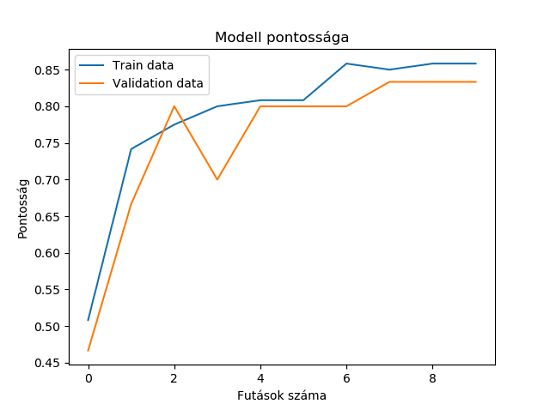
\includegraphics[scale=1]{images/accuracy.png}
\caption{A modell pontossága}
\label{fig:accuracy}
\end{figure}

\begin{figure}[h!]
\centering
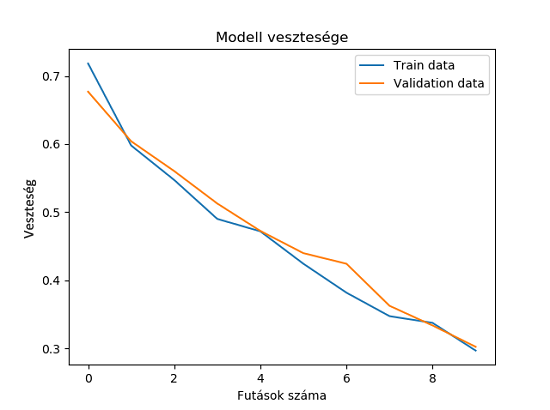
\includegraphics[scale=1]{images/loss.png}
\caption{A modell vesztesége}
\label{fig:loss}
\end{figure}

Jól látható, hogy a futások számával növekszik a pontosság és csökken a veszteség. A modell a mintákat 85\% feletti pontossággal tudta beazonosítani a 10. futás során. Ez egy egészen elfogadható arány, így megkezdhetjük a program tesztelését.

\Section{Program tesztelése}

A programot átírtam úgy, hogy egymás után olvassa be a PDF-eket és mindegyiknek az eredményeit egy külön mappába mentse. Összesen 50 dokumentumot gyűjtöttem, amelyeknek különböző a méretük, struktúrájuk és a betűtípusuk. A tesztelés arra irányult, hogy kiderüljön, hogy a program mennyire stabil, milyen pontossággal nyeri ki az adatokat az adott PDF-ből, és hogy rávilágítson a program hiányosságaira. A gép paraméterei amin teszteltem: 8GB RAM, Intel(R) Core(TM) I5-9400F 2.90 GHz processzor, 64 bites Windows operációs rendszer.

\SubSection{Futási idő becslése}

A program úgy működik, hogy beolvassa az összes oldalt a memóriába, és utána egyenként dolgozza fel őket. Ez nagyban lassítja a több oldalas dokumentumok feldolgozását és a magas oldalszámú PDF-két pedig ellehetetleníti. Tapasztalatom szerint olyan 150 oldalas dokumentum az, amit még a program az adott körülmények között kiértékel. A futási sebességek \aref{fig:runtime}. ábrán láthatók.

\begin{figure}[h!]
\centering
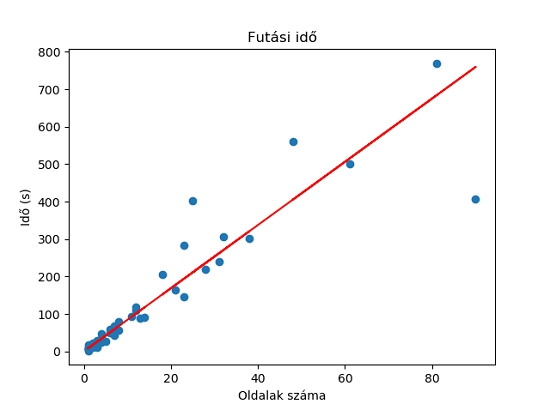
\includegraphics[scale=1]{images/runtime.png}
\caption{Futási idő a dokumentum oldalainak száma szerint}
\label{fig:runtime}
\end{figure}

Mint azt az ábra mutatja, a futási idő nem csak az oldalszámtól, hanem a PDF bonyolultságától is függ. Ezért lehetséges az, hogy egy 90 oldalas dokumentumot hamarabb feldolgozott a program mint egy 81 oldalasat. Az átlagos futási idő 8,44 másodperc/oldal volt a tesztelés során, az oldalszámok szerinti átlagot a piros vonal mutatja.

\SubSection{A paragrafusok feldolgozásának a helyessége és a szöveg helyességének a viszonya}

Mint már említettem, a paragrafusok feldolgozására épül minden más mozzanat. Mégis amit a legjobban befolyásol, az a kimeneti szövegnek a helyessége. A tesztelt dokumentumoknál a paragrafusok kivágásának a helyessége 83.99\%, míg a szövegnek 76.63\% volt. \Aref{fig:paragraph_and_text}. ábra a paragrafusok és a szöveg helyességét hasonlítja össze minden egyes dokumentumra.

\begin{figure}[h!]
\centering
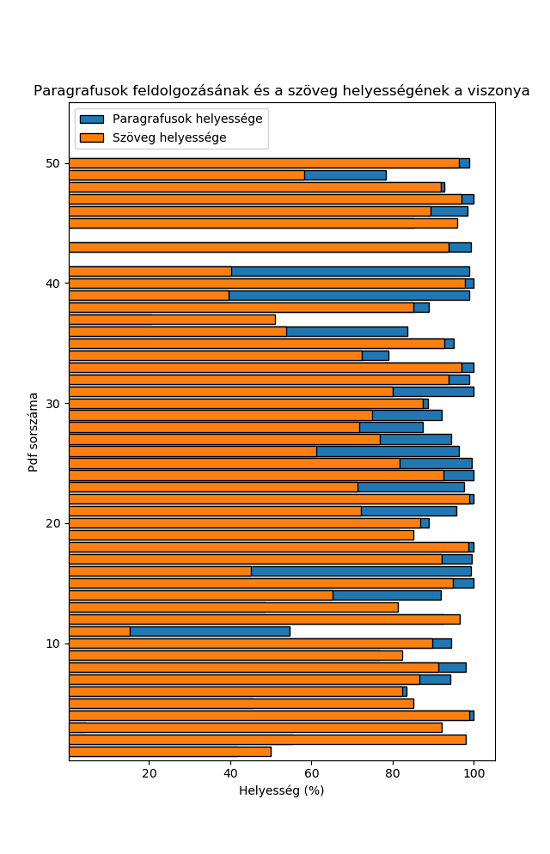
\includegraphics[scale=1]{images/paragraph_and_text.png}
\caption{A paragrafusok és a szöveg helyességének az összehasonlítása}
\label{fig:paragraph_and_text}
\end{figure}

Az ábrán jól kivehető, hogy szinte minden dokumentumra a paragrafusok feldolgozása 60\%, míg a szöveg helyessége 50\% felett volt. Két dokumentum esetében mind a kettő érték nulla, mivel az adott PDF-ek csak képeket tartalmaztak, így azok jelen esetben nem relevánsak. Az esetek 79.17\%-ban (38 esetben, a két képeket tartalmazó dokumentumokat nem számolva) ahogy romlott a paragrafusok helyességének aránya, úgy romlott vele a szöveg helyességének az aránya is. A legtöbb hiba a képek és paragrafusok megkülönböztetése miatt adódott. Szinte minden esetben előfordult, hogy legalább 1 paragrafust a képekhez, vagy egy képet a paragrafusokhoz sorolt az algoritmus.
